\chapter{Retrosynthesis and Multistep Strategy}\label{ch:b2:retrosynthesis}

A molecule is drawn on the board, and nobody yet knows how to make it. Trying reactions forwards, from
whatever is on the shelf, leads nowhere: there are too many. The chemist works the other way, from the
target back towards the shelf, cutting one bond at a time on paper, each cut undoing a reaction that is
known to work, until the pieces are compounds that can be bought. This chapter turns the reactions of
the previous chapters into that backwards reasoning, and then asks how to judge the route it produces.

\begin{recall}
\Cref{ch:b2:alkene-redox} to \cref{ch:b2:wittig}: the reactions to be undone. The Year 1 volume:
protecting groups and acetals, Grignard reagents and polarity inversion, the Williamson synthesis,
chemoselectivity, the oxidation of alcohols. The school volume: atom economy.
\end{recall}

\section{Thinking backwards}

\begin{definition}[Retrosynthetic analysis]\label{def:b2:retrosynthesis:analysis}
The molecule to be made is the \emph{target molecule}\index{target molecule}. \emph{Retrosynthetic analysis}
\index{retrosynthetic analysis} works from the target back to available starting materials,
by steps each of which is the reverse of a known reaction; a retrosynthetic step is written with the
double arrow $\Rightarrow$, read ``is made from''.
\end{definition}

\begin{definition}[Disconnection and synthons]\label{def:b2:retrosynthesis:disconnection}
A \emph{disconnection}\index{disconnection} is the imaginary cutting of a bond of the target, the
reverse of a bond-forming reaction. Cutting a bond heterolytically gives two \emph{synthons}\index{synthon},
idealised charged fragments, one a donor (nucleophilic, often negative), the other an acceptor
(electrophilic, often positive). A \emph{synthetic equivalent}\index{synthetic equivalent} is a real
reagent that behaves as a synthon: a Grignard reagent for the carbanion \ce{R-}, an aldehyde for the
cation $\mathrm{R\overset{+}{C}H{-}OH}$.
\end{definition}

\begin{definition}[Functional-group interconversion]\label{def:b2:retrosynthesis:fgi}
A \emph{functional-group interconversion}\index{functional-group interconversion} (FGI) is a
retrosynthetic step that changes a functional group without changing the carbon skeleton: an alcohol
from a ketone (by reduction), an alkane chain from an alkene (by hydrogenation), an amine from an amide.
\end{definition}

\begin{omfigure}
\begin{tikzpicture}[every node/.style={align=center}]
\node (T) at (0,0) {\setchemfig{atom sep=1.7em}\chemfig{Ph-CH(-[2]OH)-CH(-[6]CH_3)-CH_3}};
\node (A) at (-4.6,-2.6) {\ce{PhCHO}\\[1pt] + \ce{(CH3)2CHMgBr}};
\node (B) at (0,-2.6) {\ce{PhMgBr}\\[1pt] + \ce{(CH3)2CHCHO}};
\node (C) at (4.6,-2.6) {\setchemfig{atom sep=1.7em}\chemfig{Ph-C(=[2]O)-CH(-[6]CH_3)-CH_3}};
\node (D) at (4.6,-5.0) {\ce{C6H6}\\[1pt] + \ce{(CH3)2CHCOCl}};
\draw[omretro] (T.south west) -- node[above left, font=\small] {a} (A.north);
\draw[omretro] (T.south) -- node[right, font=\small] {b} (B.north);
\draw[omretro] (T.south east) -- node[above right, font=\small] {FGI} (C.north);
\draw[omretro] (C.south) -- node[right, font=\small] {c} (D.north);
\end{tikzpicture}
\par\vspace{6pt}

{\small A retrosynthetic tree for 2-methyl-1-phenylpropan-1-ol. (a) and (b): the two \omterm{def:b2:retrosynthesis:disconnection}{disconnections} of
the \ce{C-C} bond next to the alcohol carbon, each an aldehyde and a Grignard reagent. FGI: the alcohol
from a ketone, by reduction; (c) the ketone by \omterm{def:b2:aromatic-substitution:friedel-crafts}{Friedel--Crafts acylation} of benzene. Every arrow
reads ``is made from''.}
\end{omfigure}

The tree shows the habits of the method. A \omterm{def:b2:retrosynthesis:disconnection}{disconnection} is chosen at a bond next to a functional
group, because that is where reactions make bonds. Each cut is checked by writing the \omterm{def:b2:retrosynthesis:disconnection}{synthons} and
finding real reagents for them. And there is rarely one answer: the tree branches, and the branches are
judged at the end (\cref{sec:b2:retrosynthesis:judging}).

\begin{omfigure}
\begin{center}
\small
\renewcommand{\arraystretch}{1.25}
\begin{tabular}{lll}
\hline
\omterm{def:b2:retrosynthesis:disconnection}{Synthon} & Kind & \omterm{def:b2:retrosynthesis:disconnection}{Synthetic equivalent} \\
\hline
\ce{R-} (alkyl, aryl) & donor & \ce{RMgBr}, \ce{RLi}, \ce{R2CuLi} (conjugate) \\
$\mathrm{^-CH_2COR}$ & donor & the \omterm{def:b2:enolates-aldol:enolate}{enolate} of \ce{CH3COR}, or ethyl 3-oxobutanoate \\
$\mathrm{^-C{\equiv}N}$ & donor & \ce{NaCN} \\
$\mathrm{R\overset{+}{C}H{-}OH}$ & acceptor & the aldehyde \ce{RCHO} \\
$\mathrm{R\overset{+}{C}{=}O}$ & acceptor & the \omterm{def:b2:acyl-substitution:derivative}{acyl chloride} \ce{RCOCl}, an ester \\
\ce{R+} (primary) & acceptor & the halide \ce{RBr} (bimolecular substitution) \\
$\mathrm{^+CH_2CH_2COR}$ & acceptor & the enone \ce{CH2=CHCOR} (\omterm{def:b2:conjugate-additions:addition-modes}{conjugate addition}) \\
\hline
\end{tabular}
\end{center}

{\small Common \omterm{def:b2:retrosynthesis:disconnection}{synthons} and their \omterm{def:b2:retrosynthesis:disconnection}{synthetic equivalents}. The donor \omterm{def:b2:retrosynthesis:disconnection}{synthons} are carbanions, the
acceptor \omterm{def:b2:retrosynthesis:disconnection}{synthons} carbocations; the real reagents carry the same polarity without the full charge.}
\end{omfigure}

\section{One-group disconnections}

A one-group \omterm{def:b2:retrosynthesis:disconnection}{disconnection} cuts a bond next to a single functional group. For a \ce{C-O} or \ce{C-N}
bond of an ether, ester or amine, the cut goes between carbon and the heteroatom: the heteroatom is
the donor, the carbon the acceptor (a Williamson synthesis, an \omterm{def:b2:acyl-substitution:esterification}{esterification}, an amide formation).
For a \ce{C-C} bond, the functional group fixes the polarity of the \omterm{def:b2:retrosynthesis:disconnection}{synthons}: next to an alcohol
carbon, the alcohol carbon is the acceptor (an aldehyde or ketone) and the other carbon the donor (an
organometallic); next to a carbonyl, the $\alpha$ carbon is the donor (an \omterm{def:b2:enolates-aldol:enolate}{enolate}).

Most of these reactions need the right oxidation level at the right place, so FGIs between oxidation
levels are the commonest steps of a route: alkene, alcohol, aldehyde or ketone, acid. One of them was
left open in the Year 1 volume: stopping the oxidation of a primary alcohol at the aldehyde.

\begin{proposition}[Mild oxidations]\label{prop:b2:retrosynthesis:mild-oxidation}
A primary alcohol is oxidised to the aldehyde, without going on to the acid, by an oxidant used in an
anhydrous organic solvent: pyridinium chlorochromate in dichloromethane, the Swern oxidation (dimethyl
sulfoxide activated by oxalyl chloride, then triethylamine, at low temperature) or the Dess--Martin
periodinane. In water, chromium(VI) or permanganate oxidise it to the carboxylic acid.
\end{proposition}

\begin{proof}[Argument]
These oxidants remove the hydrogen of the \ce{C-H} bond on the carbon bearing an \ce{OH}. The aldehyde
formed has no such group. In water, however, an aldehyde is in equilibrium with its hydrate
\ce{RCH(OH)2}, which again has an \ce{OH} on a carbon carrying a hydrogen: the hydrate is oxidised
like an alcohol, to the acid. Without water no hydrate forms, and the oxidation stops at the
aldehyde.
\end{proof}

\section{Two-group disconnections}

When the target has two functional groups, the best \omterm{def:b2:retrosynthesis:disconnection}{disconnection} usually uses both: the bond is cut
so that one group directs the donor and the other the acceptor. The distance between the groups,
counted in carbons from one functionalised carbon to the other inclusive, tells which reaction to use.

\begin{proposition}[Patterns and their reactions]\label{prop:b2:retrosynthesis:patterns}
The relationships between two groups map onto the reactions of the previous chapters as follows. The
odd relationships (1,3 and 1,5) match the natural polarities of carbonyl chemistry; the even ones (1,4
and 1,6) do not, and need polarity inversion or the cleavage of a ring.
\end{proposition}


\begin{proof}[Argument]
In carbonyl chemistry the carbonyl carbon is an acceptor and the $\alpha$ carbon a donor, and an enone
adds an acceptor at its $\beta$ carbon. An \omterm{def:b2:enolates-aldol:enolate}{enolate} (donor at $\alpha$) on a carbonyl (acceptor at the
carbonyl carbon) joins carbons 1 and 2 of a 1,3 pattern: \omterm{def:b2:enolates-aldol:aldol}{aldol} and Claisen. An \omterm{def:b2:enolates-aldol:enolate}{enolate} on the $\beta$
carbon of an enone builds a 1,5 pattern: Michael, then Robinson. For a 1,4 pattern, the cut leaves an
$\alpha$ carbon as acceptor; no ordinary carbonyl reagent offers that polarity, but an $\alpha$-bromo
ketone does, since bromide is a leaving group at that carbon. A 1,6 dicarbonyl is a cyclohexene opened
by \omterm{def:b2:alkene-redox:cleavage}{ozonolysis} (\cref{prop:b2:alkene-redox:ozonolysis}), and the cyclohexene is made by a \omterm{def:b2:frontier-orbitals:diels-alder}{Diels--Alder
reaction} (\cref{def:b2:frontier-orbitals:diels-alder}).
\end{proof}

\begin{omfigure}
\begin{center}
\small
\renewcommand{\arraystretch}{1.25}
\begin{tabular}{lll}
\hline
Pattern in the target & \omterm{def:b2:retrosynthesis:disconnection}{Disconnection} & Reaction \\
\hline
$\beta$-hydroxy carbonyl (1,3) & $\alpha$--$\beta$ bond & \omterm{def:b2:enolates-aldol:aldol}{aldol addition} \\
$\alpha,\beta$-unsaturated carbonyl & \ce{C=C} & \omterm{def:b2:enolates-aldol:aldol}{aldol condensation} \\
1,3-dicarbonyl & C(O)--C$\alpha$ & \omterm{def:b2:enolates-aldol:claisen}{Claisen condensation} \\
1,5-dicarbonyl & C$\alpha$--C$\beta$ of the acceptor & \omterm{def:b2:conjugate-additions:michael}{Michael addition} \\
cyclohex-2-en-1-one & ring \ce{C=C}, then Michael bond & \omterm{def:b2:conjugate-additions:robinson}{Robinson annulation} \\
cyclohexene & two ring \ce{C-C} bonds & \omterm{def:b2:frontier-orbitals:diels-alder}{Diels--Alder reaction} \\
alkene at a defined place & \ce{C=C} & Wittig or HWE reaction \\
1,4-dicarbonyl & central \ce{C-C} & \omterm{def:b2:enolates-aldol:enolate}{enolate} + $\alpha$-halo ketone \\
1,6-dicarbonyl & reconnect the ends & \omterm{def:b2:alkene-redox:cleavage}{oxidative cleavage} of a cyclohexene \\
\hline
\end{tabular}
\end{center}

{\small The two-group \omterm{def:b2:retrosynthesis:disconnection}{disconnections}. The first six use the normal polarity: an \omterm{def:b2:enolates-aldol:enolate}{enolate} (donor) on a
carbonyl or an enone (acceptor). The 1,4 pattern needs a carbon $\alpha$ to a carbonyl to be the
acceptor, the reverse of its usual role, which an $\alpha$-halo ketone provides.}
\end{omfigure}

\begin{method}[A retrosynthetic analysis]\label{met:b2:retrosynthesis:retrosynthesis}
\begin{enumerate}
  \item List the functional groups of the target and their relationships (1,2; 1,3; \dots).
  \item Consider FGIs that would give a pattern with a good \omterm{def:b2:retrosynthesis:disconnection}{disconnection} (an alcohol from a ketone, an
        alkane chain from an alkene).
  \item Choose strategic bonds: next to a functional group, near the middle of the molecule, at a
        branch point or joining a ring to a chain, so that the pieces are of similar size.
  \item Write the \omterm{def:b2:retrosynthesis:disconnection}{synthons}, then their \omterm{def:b2:retrosynthesis:disconnection}{synthetic equivalents}; reject a cut with no real reagent.
  \item Check chemoselectivity: which other group would react with each reagent? Plan a protection
        or change the order of the steps.
  \item Repeat on each piece until all are available; then write the route forwards, with reagents and
        conditions.
\end{enumerate}
\end{method}

\section{Protecting groups in a route}

A route often needs a reagent that would attack a second group of the molecule. The Year 1 volume
protected aldehydes and ketones as acetals. A route chooses among several protecting groups, each
removed by its own conditions: acetals (removed by aqueous acid), silyl ethers of alcohols (removed by
fluoride ion), benzyl ethers (removed by hydrogenolysis over palladium), carbamates of amines such as
the \textit{tert}-butoxycarbonyl group (removed by acid), and esters (removed by base).

\begin{definition}[Orthogonal protection]\label{def:b2:retrosynthesis:orthogonal}
A set of \emph{orthogonal protecting groups}\index{orthogonal protecting groups} is a set of protecting
groups each removable by conditions that leave all the others intact, so that the functions they mask
can be released one at a time, in any order.
\end{definition}

\begin{method}[Protecting in a route]\label{met:b2:retrosynthesis:protect-in-route}
\begin{enumerate}
  \item For each step, list the groups the reagent would attack besides the intended one.
  \item First try to avoid protection: change the order of the steps, or use a more selective reagent
        (a borohydride instead of a hydride for a ketone beside an ester).
  \item Otherwise choose a group stable in every step until its removal, and removable in conditions the
        molecule tolerates.
  \item With several groups to release separately, choose an orthogonal set.
  \item Look for a step that removes a group for free: a hydrogenation planned anyway also removes a
        benzyl ether.
  \item Count: each protection costs two steps and their yields.
\end{enumerate}
\end{method}

\section{Judging a route}\label{sec:b2:retrosynthesis:judging}

\begin{proposition}[Overall yield]\label{prop:b2:retrosynthesis:overall-yield}
The overall yield of a linear sequence of steps is the product of the step yields:
$\rho = \rho_1 \rho_2 \cdots \rho_n$. With $n$ steps of equal yield $\rho_1$, $\rho = \rho_1^{\,n}$.
\end{proposition}

\begin{proof}
Step $k$ converts the amount $n_{k-1}$ of its starting material into $n_k = \rho_k\, n_{k-1}$ of product
(yields taken on amounts of the intermediate, all other reagents in sufficient quantity). By induction,
$n_n = \rho_n \rho_{n-1} \cdots \rho_1\, n_0$, and the overall yield $n_n/n_0$ is the product.
\end{proof}

\begin{omfigure}
\begin{tikzpicture}
\begin{axis}[width=0.75\linewidth, height=5.4cm, xmin=0, xmax=20, ymin=0, ymax=100,
  xlabel={number of steps $n$}, ylabel={overall yield (\%)}, label style={font=\small},
  tick label style={font=\scriptsize}, xtick={0,5,10,15,20}, grid=major, grid style={black!12},
  legend style={font=\scriptsize, at={(0.98,0.98)}, anchor=north east}, legend cell align=left]
\addplot[omDef, thick] table[x=n, y=r95] {figdata/out/bachelor-2-overall-yield.dat};
\addplot[omThm, thick] table[x=n, y=r90] {figdata/out/bachelor-2-overall-yield.dat};
\addplot[omMeth, thick] table[x=n, y=r80] {figdata/out/bachelor-2-overall-yield.dat};
\addplot[black!60, thick, dashed] table[x=n, y=r70] {figdata/out/bachelor-2-overall-yield.dat};
\legend{95~\% per step, 90~\% per step, 80~\% per step, 70~\% per step}
\end{axis}
\end{tikzpicture}
\par\vspace{4pt}

{\small Overall yield of a linear route against its number of steps, for four step yields
(\cref{prop:b2:retrosynthesis:overall-yield}). Ten steps at 90~\% each keep 35~\% of the material; ten
steps at 70~\%, less than 3~\%.}
% figdata: bachelor-2/overall-yield.py
\end{omfigure}

The product rule is why short routes win, why a protection (two extra steps) is never free, and why
chemists prefer to build two halves separately and join them late: the long route then runs in two
shorter branches, and the losses of one branch do not multiply those of the other. Besides yield and
length, a route is judged on \omterm{def:b2:continuous-reactors:selectivity}{selectivity} (each step should give one product), on the cost and hazard
of its reagents, on the waste it produces (the atom economy of each step and the solvents of the
purifications), and on how easily each step scales up.

\begin{history}[Working backwards, made explicit]
\begin{minipage}[t]{0.2\linewidth}
\vspace{0pt}
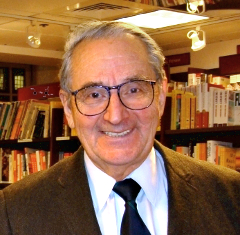
\includegraphics[width=\linewidth]{images/book3/corey.jpg}
\end{minipage}\hfill
\begin{minipage}[t]{0.76\linewidth}
\vspace{0pt}
Chemists had always reasoned backwards from their targets, but Elias James Corey, from the 1960s,
turned the habit into explicit rules: the \omterm{def:b2:retrosynthesis:disconnection}{disconnection}, the \omterm{def:b2:retrosynthesis:disconnection}{synthon}, the retrosynthetic arrow, and
even computer programs that applied them. He received the 1990 Nobel Prize in Chemistry for the theory
and methodology of organic synthesis. (Photograph: by Trvthchem, CC0, Wikimedia Commons.)
\end{minipage}
\end{history}

\begin{safety}{\ghs[5mm]{GHS02}\,\ghs[5mm]{GHS03}\,\ghs[5mm]{GHS05}\,\ghs[5mm]{GHS06}\,\ghs[5mm]{GHS07}\,\ghs[5mm]{GHS08}}
Oxalyl chloride is corrosive, toxic and reacts with water, releasing hydrogen chloride; the Swern
oxidation releases carbon monoxide and foul-smelling dimethyl sulfide, so it is run in a fume hood.
The Dess--Martin periodinane is an oxidiser and must not be heated. Chromium(VI) reagents are now
avoided where an alternative exists.
% ledger: ghs:oxalyl-chloride, ghs:DMSO, ghs:DMP
\end{safety}

\section{Exercises}

\begin{exercise}[$\star$]\label{exo:b2:retrosynthesis:1}
Disconnect each alcohol into a carbonyl compound and a Grignard reagent (give every possibility):
2-phenylpropan-2-ol, pentan-3-ol, 1-cyclohexylethanol, 2-methylbutan-2-ol, 1-phenylethanol.
\end{exercise}

\begin{exercise}[$\star$]\label{exo:b2:retrosynthesis:2}
For the \omterm{def:b2:retrosynthesis:disconnection}{disconnection} of 1-phenylethanol at the \ce{C-C} bond, name the two \omterm{def:b2:retrosynthesis:disconnection}{synthons}, say which is the
donor, and give a \omterm{def:b2:retrosynthesis:disconnection}{synthetic equivalent} for each.
\end{exercise}

\begin{exercise}[$\star$]\label{exo:b2:retrosynthesis:3}
A five-step route has step yields of 90, 85, 80, 95 and 70~\%. Compute its overall yield.
\end{exercise}

\begin{exercise}[$\star$]\label{exo:b2:retrosynthesis:4}
Ethyl 4-oxopentanoate must be turned into 5-hydroxypentan-2-one. Plan the route with a protecting
group, and say why it is needed.
\end{exercise}

\begin{exercise}[$\star\star$]\label{exo:b2:retrosynthesis:5}
Propose a retrosynthesis of butane-1,3-diol from compounds with at most two carbons, with an FGI and a
two-group \omterm{def:b2:retrosynthesis:disconnection}{disconnection}.
\end{exercise}

\begin{exercise}[$\star\star$]\label{exo:b2:retrosynthesis:6}
Disconnect 1-(cyclohex-3-en-1-yl)ethan-1-one by a \omterm{def:b2:frontier-orbitals:diels-alder}{Diels--Alder reaction}.
\end{exercise}

\begin{exercise}[$\star\star$]\label{exo:b2:retrosynthesis:7}
Disconnect 4,4-dimethylcyclohex-2-en-1-one by a \omterm{def:b2:conjugate-additions:robinson}{Robinson annulation}.
\end{exercise}

\begin{exercise}[$\star\star$]\label{exo:b2:retrosynthesis:8}
1-Phenylbutan-1-one can be made in one step by a \omterm{def:b2:aromatic-substitution:friedel-crafts}{Friedel--Crafts acylation}, or in two from benzaldehyde.
Write both routes and compare them.
\end{exercise}

\begin{exercise}[$\star\star$]\label{exo:b2:retrosynthesis:9}
Hexanal is wanted from hexan-1-ol. Which reagents give it, and which one would give hexanoic acid
instead? Explain.
\end{exercise}

\begin{exercise}[$\star\star\star$]\label{exo:b2:retrosynthesis:10}
In 4-aminobutan-1-ol, the amine must react first with an \omterm{def:b2:acyl-substitution:derivative}{acyl chloride} in one step, and the alcohol
later with another. Propose an orthogonal pair of protecting groups and the sequence.
\end{exercise}

\begin{exercise}[$\star\star\star$]\label{exo:b2:retrosynthesis:11}
Propose a synthesis of hexane-2,5-dione, a 1,4-dicarbonyl compound, from ethyl 3-oxobutanoate.
\end{exercise}

\begin{exercise}[$\star\star\star$]\label{exo:b2:retrosynthesis:12}
6-Methylhept-5-en-2-one, \ce{(CH3)2C=CHCH2CH2COCH3}, is a fragrance intermediate. Propose a full plan
from ethyl 3-oxobutanoate and a halide: retrosynthesis, forward route, and the step that removes the
ester.
\end{exercise}

\section{Problem: Raspberry Ketone}

\begin{problem}[{Weekend problem --- the retrosynthesis of a flavour compound, the phenol and whether
to protect it, a palladium alternative, and the judgement of the routes}]
\label{pb:b2:retrosynthesis:1}
Raspberry ketone, 4-(4-hydroxyphenyl)butan-2-one, is found in raspberries and other fruits and is used
as a flavouring and in perfumery. Exercise data: step yields of the \omterm{def:b2:enolates-aldol:aldol}{aldol} route, 85~\% (condensation)
and 92~\% (hydrogenation). Molar masses (\unit{g/mol}): C 12.011, H 1.008, O 15.999, N 14.007,
I 126.90. The $\mathrm pK_a$ of phenol is 9.99.
% ledger: use:raspberry-ketone, aw:C, aw:H, aw:O, aw:N, aw:I, pka:phenol, ghs:raspberry-ketone, ghs:4-iodophenol, ghs:MVK

\medskip
\noindent\textbf{Part I --- Retrosynthesis.}
\begin{enumerate}
  \item Draw the target and name its functional groups.
  \item Which FGI turns the \ce{ArCH2CH2CO} unit into a pattern with a known \omterm{def:b2:retrosynthesis:disconnection}{disconnection}?
  \item Write the unsaturated ketone obtained, with its geometry.
  \item Which two-group pattern does it contain, and which reaction makes it?
  \item Name the two starting materials.
  \item Why does this crossed \omterm{def:b2:enolates-aldol:aldol}{aldol} give one main product?
  \item Write the forward route in two steps, with conditions.
\end{enumerate}

\medskip
\noindent\textbf{Part II --- The phenol.}
\begin{enumerate}[resume]
  \item In aqueous sodium hydroxide, in which form is 4-hydroxybenzaldehyde present? Use the
        $\mathrm pK_a$.
  \item How does that form change the electrophilicity of the aldehyde?
  \item If the phenol were protected, which group would the second step remove for free? Explain.
  \item Count the steps of the route with that protection.
  \item Is the benzene ring at risk in the hydrogenation?
  \item Protect or not? Conclude.
\end{enumerate}

\medskip
\noindent\textbf{Part III --- A palladium alternative.}
\begin{enumerate}[resume]
  \item Disconnect the unsaturated ketone at the bond between the ring and the chain: which Heck
        partners?
  \item Write the Heck reaction with triethylamine as base.
  \item At which carbon of but-3-en-2-one does the aryl group end up, and why?
  \item Name the steps of the \omterm{def:b2:catalytic-cycles:cycle}{catalytic cycle}.
  \item Compute the atom economy of the Heck step, counting triethylamine.
  \item Compute the atom economy of the \omterm{def:b2:enolates-aldol:aldol}{aldol condensation}.
\end{enumerate}

\medskip
\noindent\textbf{Part IV --- Judging the routes.}
\begin{enumerate}[resume]
  \item What is the atom economy of the hydrogenation?
  \item Compute the overall atom economy of the \omterm{def:b2:enolates-aldol:aldol}{aldol} route.
  \item Which double bond does the hydrogenation reduce, and why does the ketone survive?
  \item Compare the reagents of the two routes for cost and hazard.
  \item Which route would you choose?
  \item What would a third step at 90~\% do to the overall yield?
  \item State the overall yield of the two-step \omterm{def:b2:enolates-aldol:aldol}{aldol} route.
\end{enumerate}
\end{problem}
